

% This document was generated by the publish-function
% from GNU Octave 4.2.1



\documentclass[10pt]{article}
\usepackage{listings}
\usepackage{mathtools}
\usepackage{amssymb}
\usepackage{graphicx}
\usepackage{hyperref}
\usepackage{xcolor}
\usepackage{titlesec}
\usepackage[utf8]{inputenc}
\usepackage[T1]{fontenc}
\usepackage{lmodern}


\lstset{
language=Octave,
numbers=none,
frame=single,
tabsize=2,
showstringspaces=false,
breaklines=true}


\titleformat*{\section}{\Huge\bfseries}
\titleformat*{\subsection}{\large\bfseries}
\renewcommand{\contentsname}{\Large\bfseries Contents}
\setlength{\parindent}{0pt}

\begin{document}

{\Huge\section*{aufgabe1}}

\tableofcontents
\vspace*{4em}

\begin{lstlisting}
%k soll entweder 10,50,250

prompt = 'please enter value for k:'
k = input(prompt)

%file definieren
file = 'sprech.wav'

%lesen des files in ein array
%y = sampledata
%Fs = samplerate
[y,Fs] = audioread(file);

%ausgabe der filegroesse
[samples, channels] = size (y)


%stereo -> mono
y = (y(:,1) + y(:,2))/2;
a=1;
b=(1/k)*ones(1,k);
filtered = filter(b,a,y);

y = y /max(abs(y));
filtered = filtered /max(abs(filtered));

subplot(2,1,2);
plot(filtered);
title('filtered signal')
subplot(2,1,1);
plot(y);
title('unfilterted signal')


%info inkl. samplerate
sound(y,Fs)

pause()

%abspielen der ungefilterten datei
sound(filtered,Fs)
\end{lstlisting}
\begin{lstlisting}[language={},xleftmargin=5pt,frame=none]
prompt = please enter value for k:

\end{lstlisting}
\begin{figure}[!ht]
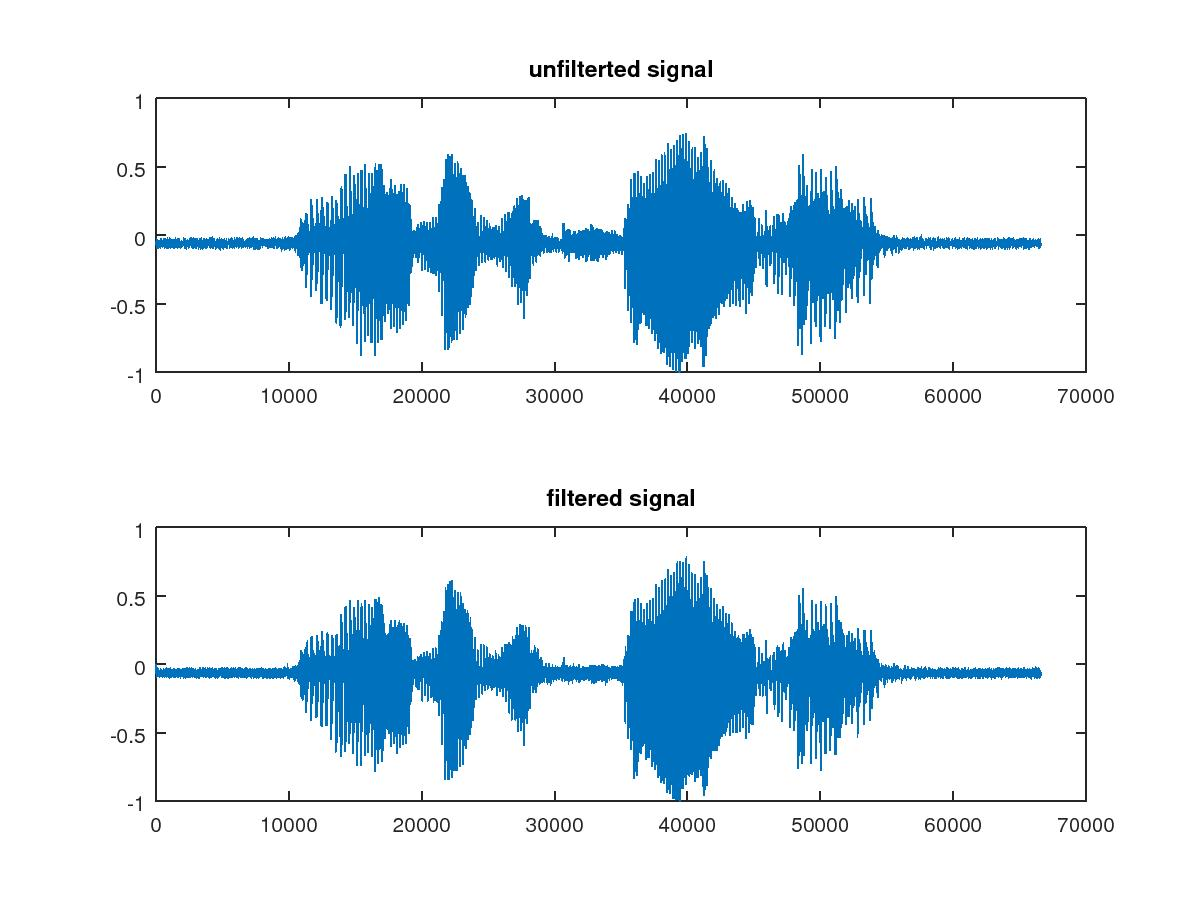
\includegraphics[width=\textwidth]{aufgabe1-1.jpg}
\end{figure}


\end{document}
